\documentclass[twoside]{book}

% Packages required by doxygen
\usepackage{fixltx2e}
\usepackage{calc}
\usepackage{doxygen}
\usepackage[export]{adjustbox} % also loads graphicx
\usepackage{graphicx}
\usepackage[utf8]{inputenc}
\usepackage{makeidx}
\usepackage{multicol}
\usepackage{multirow}
\PassOptionsToPackage{warn}{textcomp}
\usepackage{textcomp}
\usepackage[nointegrals]{wasysym}
\usepackage[table]{xcolor}

% Font selection
\usepackage[T1]{fontenc}
\usepackage[scaled=.90]{helvet}
\usepackage{courier}
\usepackage{amssymb}
\usepackage{sectsty}
\renewcommand{\familydefault}{\sfdefault}
\allsectionsfont{%
  \fontseries{bc}\selectfont%
  \color{darkgray}%
}
\renewcommand{\DoxyLabelFont}{%
  \fontseries{bc}\selectfont%
  \color{darkgray}%
}
\newcommand{\+}{\discretionary{\mbox{\scriptsize$\hookleftarrow$}}{}{}}

% Page & text layout
\usepackage{geometry}
\geometry{%
  a4paper,%
  top=2.5cm,%
  bottom=2.5cm,%
  left=2.5cm,%
  right=2.5cm%
}
\tolerance=750
\hfuzz=15pt
\hbadness=750
\setlength{\emergencystretch}{15pt}
\setlength{\parindent}{0cm}
\setlength{\parskip}{3ex plus 2ex minus 2ex}
\makeatletter
\renewcommand{\paragraph}{%
  \@startsection{paragraph}{4}{0ex}{-1.0ex}{1.0ex}{%
    \normalfont\normalsize\bfseries\SS@parafont%
  }%
}
\renewcommand{\subparagraph}{%
  \@startsection{subparagraph}{5}{0ex}{-1.0ex}{1.0ex}{%
    \normalfont\normalsize\bfseries\SS@subparafont%
  }%
}
\makeatother

% Headers & footers
\usepackage{fancyhdr}
\pagestyle{fancyplain}
\fancyhead[LE]{\fancyplain{}{\bfseries\thepage}}
\fancyhead[CE]{\fancyplain{}{}}
\fancyhead[RE]{\fancyplain{}{\bfseries\leftmark}}
\fancyhead[LO]{\fancyplain{}{\bfseries\rightmark}}
\fancyhead[CO]{\fancyplain{}{}}
\fancyhead[RO]{\fancyplain{}{\bfseries\thepage}}
\fancyfoot[LE]{\fancyplain{}{}}
\fancyfoot[CE]{\fancyplain{}{}}
\fancyfoot[RE]{\fancyplain{}{\bfseries\scriptsize Generated by Doxygen }}
\fancyfoot[LO]{\fancyplain{}{\bfseries\scriptsize Generated by Doxygen }}
\fancyfoot[CO]{\fancyplain{}{}}
\fancyfoot[RO]{\fancyplain{}{}}
\renewcommand{\footrulewidth}{0.4pt}
\renewcommand{\chaptermark}[1]{%
  \markboth{#1}{}%
}
\renewcommand{\sectionmark}[1]{%
  \markright{\thesection\ #1}%
}

% Indices & bibliography
\usepackage{natbib}
\usepackage[titles]{tocloft}
\setcounter{tocdepth}{3}
\setcounter{secnumdepth}{5}
\makeindex

% Hyperlinks (required, but should be loaded last)
\usepackage{ifpdf}
\ifpdf
  \usepackage[pdftex,pagebackref=true]{hyperref}
\else
  \usepackage[ps2pdf,pagebackref=true]{hyperref}
\fi
\hypersetup{%
  colorlinks=true,%
  linkcolor=blue,%
  citecolor=blue,%
  unicode%
}

% Custom commands
\newcommand{\clearemptydoublepage}{%
  \newpage{\pagestyle{empty}\cleardoublepage}%
}

\usepackage{caption}
\captionsetup{labelsep=space,justification=centering,font={bf},singlelinecheck=off,skip=4pt,position=top}

%===== C O N T E N T S =====

\begin{document}

% Titlepage & ToC
\hypersetup{pageanchor=false,
             bookmarksnumbered=true,
             pdfencoding=unicode
            }
\pagenumbering{alph}
\begin{titlepage}
\vspace*{7cm}
\begin{center}%
{\Large war }\\
\vspace*{1cm}
{\large Generated by Doxygen 1.8.13}\\
\end{center}
\end{titlepage}
\clearemptydoublepage
\pagenumbering{roman}
\tableofcontents
\clearemptydoublepage
\pagenumbering{arabic}
\hypersetup{pageanchor=true}

%--- Begin generated contents ---
\chapter{Data Structure Index}
\section{Data Structures}
Here are the data structures with brief descriptions\+:\begin{DoxyCompactList}
\item\contentsline{section}{\hyperlink{structbackground}{background} }{\pageref{structbackground}}{}
\item\contentsline{section}{\hyperlink{structennemi}{ennemi} }{\pageref{structennemi}}{}
\item\contentsline{section}{\hyperlink{structpersonnage}{personnage} }{\pageref{structpersonnage}}{}
\item\contentsline{section}{\hyperlink{structscore}{score} }{\pageref{structscore}}{}
\item\contentsline{section}{\hyperlink{structtimer}{timer} }{\pageref{structtimer}}{}
\item\contentsline{section}{\hyperlink{structvie}{vie} }{\pageref{structvie}}{}
\end{DoxyCompactList}

\chapter{File Index}
\section{File List}
Here is a list of all files with brief descriptions\+:\begin{DoxyCompactList}
\item\contentsline{section}{\hyperlink{main_8c}{main.\+c} }{\pageref{main_8c}}{}
\item\contentsline{section}{\hyperlink{perso_8c}{perso.\+c} }{\pageref{perso_8c}}{}
\item\contentsline{section}{\hyperlink{perso_8h}{perso.\+h} }{\pageref{perso_8h}}{}
\end{DoxyCompactList}

\chapter{Data Structure Documentation}
\hypertarget{structbackground}{}\section{background Struct Reference}
\label{structbackground}\index{background@{background}}


struct for background  




{\ttfamily \#include $<$save.\+h$>$}

\subsection*{Public Attributes}
\begin{DoxyCompactItemize}
\item 
S\+D\+L\+\_\+\+Surface $\ast$ \hyperlink{structbackground_a1c5c3a3ebb56924b9f829602f9641006}{img}
\item 
S\+D\+L\+\_\+\+Rect \hyperlink{structbackground_aa70f1467505f43c50fec228c21bd7af4}{pos}
\end{DoxyCompactItemize}


\subsection{Detailed Description}
struct for background 

\subsection{Member Data Documentation}
\index{background@{background}!img@{img}}
\index{img@{img}!background@{background}}
\subsubsection[{\texorpdfstring{img}{img}}]{\setlength{\rightskip}{0pt plus 5cm}S\+D\+L\+\_\+\+Surface$\ast$ background\+::img}\hypertarget{structbackground_a1c5c3a3ebb56924b9f829602f9641006}{}\label{structbackground_a1c5c3a3ebb56924b9f829602f9641006}
\index{background@{background}!pos@{pos}}
\index{pos@{pos}!background@{background}}
\subsubsection[{\texorpdfstring{pos}{pos}}]{\setlength{\rightskip}{0pt plus 5cm}S\+D\+L\+\_\+\+Rect background\+::pos}\hypertarget{structbackground_aa70f1467505f43c50fec228c21bd7af4}{}\label{structbackground_aa70f1467505f43c50fec228c21bd7af4}


The documentation for this struct was generated from the following file\+:\begin{DoxyCompactItemize}
\item 
\hyperlink{save_8h}{save.\+h}\end{DoxyCompactItemize}

\hypertarget{structennemi}{}\section{ennemi Struct Reference}
\label{structennemi}\index{ennemi@{ennemi}}


{\ttfamily \#include $<$save.\+h$>$}

\subsection*{Public Attributes}
\begin{DoxyCompactItemize}
\item 
S\+D\+L\+\_\+\+Rect \hyperlink{structennemi_ab236808a3af75588847442504250d02f}{position\+\_\+ennemi}
\item 
S\+D\+L\+\_\+\+Rect \hyperlink{structennemi_a1fca83eeee08fde8a80a8b9c0a0ae00f}{pos2}
\item 
S\+D\+L\+\_\+\+Rect \hyperlink{structennemi_a04c7d21c26dd2fd99eceecd6059bff90}{pos1}
\item 
S\+D\+L\+\_\+\+Rect \hyperlink{structennemi_abc473e1ffbf2e5848151d900724e3f83}{position\+\_\+sprite}
\item 
int \hyperlink{structennemi_aa1f57a616910ffd5799f1097a3160e0b}{direction}
\item 
S\+D\+L\+\_\+\+Surface $\ast$ \hyperlink{structennemi_a4f333ffffb5036c74a62a60437d60422}{spriteleft}
\item 
S\+D\+L\+\_\+\+Surface $\ast$ \hyperlink{structennemi_a8ad9de831604958b2654c033280129f1}{spriteright}
\end{DoxyCompactItemize}


\subsection{Member Data Documentation}
\index{ennemi@{ennemi}!direction@{direction}}
\index{direction@{direction}!ennemi@{ennemi}}
\subsubsection[{\texorpdfstring{direction}{direction}}]{\setlength{\rightskip}{0pt plus 5cm}int ennemi\+::direction}\hypertarget{structennemi_aa1f57a616910ffd5799f1097a3160e0b}{}\label{structennemi_aa1f57a616910ffd5799f1097a3160e0b}
\index{ennemi@{ennemi}!pos1@{pos1}}
\index{pos1@{pos1}!ennemi@{ennemi}}
\subsubsection[{\texorpdfstring{pos1}{pos1}}]{\setlength{\rightskip}{0pt plus 5cm}S\+D\+L\+\_\+\+Rect ennemi\+::pos1}\hypertarget{structennemi_a04c7d21c26dd2fd99eceecd6059bff90}{}\label{structennemi_a04c7d21c26dd2fd99eceecd6059bff90}
\index{ennemi@{ennemi}!pos2@{pos2}}
\index{pos2@{pos2}!ennemi@{ennemi}}
\subsubsection[{\texorpdfstring{pos2}{pos2}}]{\setlength{\rightskip}{0pt plus 5cm}S\+D\+L\+\_\+\+Rect ennemi\+::pos2}\hypertarget{structennemi_a1fca83eeee08fde8a80a8b9c0a0ae00f}{}\label{structennemi_a1fca83eeee08fde8a80a8b9c0a0ae00f}
\index{ennemi@{ennemi}!position\+\_\+ennemi@{position\+\_\+ennemi}}
\index{position\+\_\+ennemi@{position\+\_\+ennemi}!ennemi@{ennemi}}
\subsubsection[{\texorpdfstring{position\+\_\+ennemi}{position_ennemi}}]{\setlength{\rightskip}{0pt plus 5cm}S\+D\+L\+\_\+\+Rect ennemi\+::position\+\_\+ennemi}\hypertarget{structennemi_ab236808a3af75588847442504250d02f}{}\label{structennemi_ab236808a3af75588847442504250d02f}
\index{ennemi@{ennemi}!position\+\_\+sprite@{position\+\_\+sprite}}
\index{position\+\_\+sprite@{position\+\_\+sprite}!ennemi@{ennemi}}
\subsubsection[{\texorpdfstring{position\+\_\+sprite}{position_sprite}}]{\setlength{\rightskip}{0pt plus 5cm}S\+D\+L\+\_\+\+Rect ennemi\+::position\+\_\+sprite}\hypertarget{structennemi_abc473e1ffbf2e5848151d900724e3f83}{}\label{structennemi_abc473e1ffbf2e5848151d900724e3f83}
\index{ennemi@{ennemi}!spriteleft@{spriteleft}}
\index{spriteleft@{spriteleft}!ennemi@{ennemi}}
\subsubsection[{\texorpdfstring{spriteleft}{spriteleft}}]{\setlength{\rightskip}{0pt plus 5cm}S\+D\+L\+\_\+\+Surface$\ast$ ennemi\+::spriteleft}\hypertarget{structennemi_a4f333ffffb5036c74a62a60437d60422}{}\label{structennemi_a4f333ffffb5036c74a62a60437d60422}
\index{ennemi@{ennemi}!spriteright@{spriteright}}
\index{spriteright@{spriteright}!ennemi@{ennemi}}
\subsubsection[{\texorpdfstring{spriteright}{spriteright}}]{\setlength{\rightskip}{0pt plus 5cm}S\+D\+L\+\_\+\+Surface$\ast$ ennemi\+::spriteright}\hypertarget{structennemi_a8ad9de831604958b2654c033280129f1}{}\label{structennemi_a8ad9de831604958b2654c033280129f1}


The documentation for this struct was generated from the following file\+:\begin{DoxyCompactItemize}
\item 
\hyperlink{save_8h}{save.\+h}\end{DoxyCompactItemize}

\hypertarget{structpersonnage}{}\section{personnage Struct Reference}
\label{structpersonnage}\index{personnage@{personnage}}


{\ttfamily \#include $<$struct.\+h$>$}



Collaboration diagram for personnage\+:
\nopagebreak
\begin{figure}[H]
\begin{center}
\leavevmode
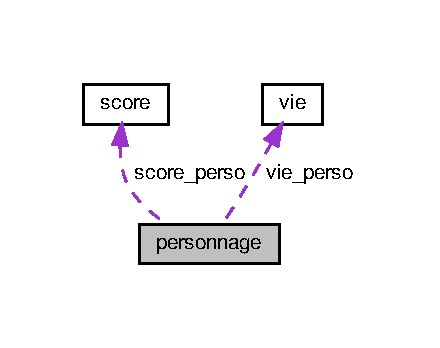
\includegraphics[width=211pt]{structpersonnage__coll__graph}
\end{center}
\end{figure}
\subsection*{Data Fields}
\begin{DoxyCompactItemize}
\item 
S\+D\+L\+\_\+\+Surface $\ast$ \hyperlink{structpersonnage_a3fc8b5a6848cc4b09b844f482411a414}{sprite} \mbox{[}12\mbox{]}
\item 
S\+D\+L\+\_\+\+Rect \hyperlink{structpersonnage_a4a45c9e4310d819fcd3c9a60fc8c0ebf}{position\+\_\+perso}
\item 
int \hyperlink{structpersonnage_a2664acffa6fccd8487b9e03b63fbd6da}{direction}
\item 
\hyperlink{structvie}{vie} \hyperlink{structpersonnage_ac96f4aee44111bc31a7718e5762bf483}{vie\+\_\+perso}
\item 
\hyperlink{structscore}{score} \hyperlink{structpersonnage_a7ea99b7d0c8445cb3d7ba6717eb89d8c}{score\+\_\+perso}
\item 
int \hyperlink{structpersonnage_acfac32928075716cc10265cfc9f551fc}{num}
\end{DoxyCompactItemize}


\subsection{Field Documentation}
\mbox{\Hypertarget{structpersonnage_a2664acffa6fccd8487b9e03b63fbd6da}\label{structpersonnage_a2664acffa6fccd8487b9e03b63fbd6da}} 
\index{personnage@{personnage}!direction@{direction}}
\index{direction@{direction}!personnage@{personnage}}
\subsubsection{\texorpdfstring{direction}{direction}}
{\footnotesize\ttfamily int personnage\+::direction}

\mbox{\Hypertarget{structpersonnage_acfac32928075716cc10265cfc9f551fc}\label{structpersonnage_acfac32928075716cc10265cfc9f551fc}} 
\index{personnage@{personnage}!num@{num}}
\index{num@{num}!personnage@{personnage}}
\subsubsection{\texorpdfstring{num}{num}}
{\footnotesize\ttfamily int personnage\+::num}

\mbox{\Hypertarget{structpersonnage_a4a45c9e4310d819fcd3c9a60fc8c0ebf}\label{structpersonnage_a4a45c9e4310d819fcd3c9a60fc8c0ebf}} 
\index{personnage@{personnage}!position\+\_\+perso@{position\+\_\+perso}}
\index{position\+\_\+perso@{position\+\_\+perso}!personnage@{personnage}}
\subsubsection{\texorpdfstring{position\+\_\+perso}{position\_perso}}
{\footnotesize\ttfamily S\+D\+L\+\_\+\+Rect personnage\+::position\+\_\+perso}

\mbox{\Hypertarget{structpersonnage_a7ea99b7d0c8445cb3d7ba6717eb89d8c}\label{structpersonnage_a7ea99b7d0c8445cb3d7ba6717eb89d8c}} 
\index{personnage@{personnage}!score\+\_\+perso@{score\+\_\+perso}}
\index{score\+\_\+perso@{score\+\_\+perso}!personnage@{personnage}}
\subsubsection{\texorpdfstring{score\+\_\+perso}{score\_perso}}
{\footnotesize\ttfamily \hyperlink{structscore}{score} personnage\+::score\+\_\+perso}

\mbox{\Hypertarget{structpersonnage_a3fc8b5a6848cc4b09b844f482411a414}\label{structpersonnage_a3fc8b5a6848cc4b09b844f482411a414}} 
\index{personnage@{personnage}!sprite@{sprite}}
\index{sprite@{sprite}!personnage@{personnage}}
\subsubsection{\texorpdfstring{sprite}{sprite}}
{\footnotesize\ttfamily S\+D\+L\+\_\+\+Surface$\ast$ personnage\+::sprite\mbox{[}12\mbox{]}}

\mbox{\Hypertarget{structpersonnage_ac96f4aee44111bc31a7718e5762bf483}\label{structpersonnage_ac96f4aee44111bc31a7718e5762bf483}} 
\index{personnage@{personnage}!vie\+\_\+perso@{vie\+\_\+perso}}
\index{vie\+\_\+perso@{vie\+\_\+perso}!personnage@{personnage}}
\subsubsection{\texorpdfstring{vie\+\_\+perso}{vie\_perso}}
{\footnotesize\ttfamily \hyperlink{structvie}{vie} personnage\+::vie\+\_\+perso}



The documentation for this struct was generated from the following file\+:\begin{DoxyCompactItemize}
\item 
\hyperlink{struct_8h}{struct.\+h}\end{DoxyCompactItemize}

\hypertarget{structscore}{}\section{score Struct Reference}
\label{structscore}\index{score@{score}}


struct for score of hero  




{\ttfamily \#include $<$perso.\+h$>$}

\subsection*{Public Attributes}
\begin{DoxyCompactItemize}
\item 
int \hyperlink{structscore_a86ee1f22a5bf4e92781f2b2165aa0859}{score\+\_\+atteint}
\item 
S\+D\+L\+\_\+\+Rect \hyperlink{structscore_a444e826e64d1abf14dc0108095752cc1}{position\+\_\+score}
\item 
T\+T\+F\+\_\+\+Font $\ast$ \hyperlink{structscore_aa8088c00f0a0ce91db39deb03afc7110}{police\+\_\+score}
\item 
S\+D\+L\+\_\+\+Surface $\ast$ \hyperlink{structscore_aa5918332d1797da4bedaccfce5446b88}{score\+\_\+texte}
\end{DoxyCompactItemize}


\subsection{Detailed Description}
struct for score of hero 

\subsection{Member Data Documentation}
\index{score@{score}!police\+\_\+score@{police\+\_\+score}}
\index{police\+\_\+score@{police\+\_\+score}!score@{score}}
\subsubsection[{\texorpdfstring{police\+\_\+score}{police_score}}]{\setlength{\rightskip}{0pt plus 5cm}T\+T\+F\+\_\+\+Font$\ast$ score\+::police\+\_\+score}\hypertarget{structscore_aa8088c00f0a0ce91db39deb03afc7110}{}\label{structscore_aa8088c00f0a0ce91db39deb03afc7110}
font \index{score@{score}!position\+\_\+score@{position\+\_\+score}}
\index{position\+\_\+score@{position\+\_\+score}!score@{score}}
\subsubsection[{\texorpdfstring{position\+\_\+score}{position_score}}]{\setlength{\rightskip}{0pt plus 5cm}S\+D\+L\+\_\+\+Rect score\+::position\+\_\+score}\hypertarget{structscore_a444e826e64d1abf14dc0108095752cc1}{}\label{structscore_a444e826e64d1abf14dc0108095752cc1}
rectangle \index{score@{score}!score\+\_\+atteint@{score\+\_\+atteint}}
\index{score\+\_\+atteint@{score\+\_\+atteint}!score@{score}}
\subsubsection[{\texorpdfstring{score\+\_\+atteint}{score_atteint}}]{\setlength{\rightskip}{0pt plus 5cm}int score\+::score\+\_\+atteint}\hypertarget{structscore_a86ee1f22a5bf4e92781f2b2165aa0859}{}\label{structscore_a86ee1f22a5bf4e92781f2b2165aa0859}
entier \index{score@{score}!score\+\_\+texte@{score\+\_\+texte}}
\index{score\+\_\+texte@{score\+\_\+texte}!score@{score}}
\subsubsection[{\texorpdfstring{score\+\_\+texte}{score_texte}}]{\setlength{\rightskip}{0pt plus 5cm}S\+D\+L\+\_\+\+Surface$\ast$ score\+::score\+\_\+texte}\hypertarget{structscore_aa5918332d1797da4bedaccfce5446b88}{}\label{structscore_aa5918332d1797da4bedaccfce5446b88}
surface 

The documentation for this struct was generated from the following file\+:\begin{DoxyCompactItemize}
\item 
\hyperlink{perso_8h}{perso.\+h}\end{DoxyCompactItemize}

\hypertarget{structtimer}{}\section{timer Struct Reference}
\label{structtimer}\index{timer@{timer}}


{\ttfamily \#include $<$horloge.\+h$>$}

\subsection*{Data Fields}
\begin{DoxyCompactItemize}
\item 
int \hyperlink{structtimer_ab6e316bed36d7d86f4c326a2bff3f989}{min}
\item 
int \hyperlink{structtimer_adf1c1abd803dda0b69234217f0e25199}{sec}
\end{DoxyCompactItemize}


\subsection{Field Documentation}
\mbox{\Hypertarget{structtimer_ab6e316bed36d7d86f4c326a2bff3f989}\label{structtimer_ab6e316bed36d7d86f4c326a2bff3f989}} 
\index{timer@{timer}!min@{min}}
\index{min@{min}!timer@{timer}}
\subsubsection{\texorpdfstring{min}{min}}
{\footnotesize\ttfamily int timer\+::min}

\mbox{\Hypertarget{structtimer_adf1c1abd803dda0b69234217f0e25199}\label{structtimer_adf1c1abd803dda0b69234217f0e25199}} 
\index{timer@{timer}!sec@{sec}}
\index{sec@{sec}!timer@{timer}}
\subsubsection{\texorpdfstring{sec}{sec}}
{\footnotesize\ttfamily int timer\+::sec}



The documentation for this struct was generated from the following file\+:\begin{DoxyCompactItemize}
\item 
\hyperlink{horloge_8h}{horloge.\+h}\end{DoxyCompactItemize}

\hypertarget{structvie}{}\section{vie Struct Reference}
\label{structvie}\index{vie@{vie}}


struct for vie perso  




{\ttfamily \#include $<$save.\+h$>$}

\subsection*{Public Attributes}
\begin{DoxyCompactItemize}
\item 
int \hyperlink{structvie_ace0f84a19ce4f5854ec56c137b33b947}{nbredevie}
\item 
S\+D\+L\+\_\+\+Surface $\ast$ \hyperlink{structvie_a2c29f60898de16e1306bd1043fa38dc9}{vie} \mbox{[}4\mbox{]}
\item 
S\+D\+L\+\_\+\+Rect \hyperlink{structvie_aaa37f269f7261984f2e540534210af5a}{position\+\_\+de\+\_\+vie}
\end{DoxyCompactItemize}


\subsection{Detailed Description}
struct for vie perso 

\subsection{Member Data Documentation}
\index{vie@{vie}!nbredevie@{nbredevie}}
\index{nbredevie@{nbredevie}!vie@{vie}}
\subsubsection[{\texorpdfstring{nbredevie}{nbredevie}}]{\setlength{\rightskip}{0pt plus 5cm}int vie\+::nbredevie}\hypertarget{structvie_ace0f84a19ce4f5854ec56c137b33b947}{}\label{structvie_ace0f84a19ce4f5854ec56c137b33b947}
entier \index{vie@{vie}!position\+\_\+de\+\_\+vie@{position\+\_\+de\+\_\+vie}}
\index{position\+\_\+de\+\_\+vie@{position\+\_\+de\+\_\+vie}!vie@{vie}}
\subsubsection[{\texorpdfstring{position\+\_\+de\+\_\+vie}{position_de_vie}}]{\setlength{\rightskip}{0pt plus 5cm}S\+D\+L\+\_\+\+Rect vie\+::position\+\_\+de\+\_\+vie}\hypertarget{structvie_aaa37f269f7261984f2e540534210af5a}{}\label{structvie_aaa37f269f7261984f2e540534210af5a}
rectangle \index{vie@{vie}!vie@{vie}}
\index{vie@{vie}!vie@{vie}}
\subsubsection[{\texorpdfstring{vie}{vie}}]{\setlength{\rightskip}{0pt plus 5cm}S\+D\+L\+\_\+\+Surface$\ast$ vie\+::vie\mbox{[}4\mbox{]}}\hypertarget{structvie_a2c29f60898de16e1306bd1043fa38dc9}{}\label{structvie_a2c29f60898de16e1306bd1043fa38dc9}
surface 

The documentation for this struct was generated from the following file\+:\begin{DoxyCompactItemize}
\item 
\hyperlink{save_8h}{save.\+h}\end{DoxyCompactItemize}

\chapter{File Documentation}
\hypertarget{animennemi_8c}{}\section{animennemi.\+c File Reference}
\label{animennemi_8c}\index{animennemi.\+c@{animennemi.\+c}}
{\ttfamily \#include \char`\"{}animennemi.\+h\char`\"{}}\newline
{\ttfamily \#include $<$stdio.\+h$>$}\newline
{\ttfamily \#include $<$stdlib.\+h$>$}\newline
{\ttfamily \#include \char`\"{}S\+D\+L/\+S\+D\+L.\+h\char`\"{}}\newline
{\ttfamily \#include \char`\"{}S\+D\+L/\+S\+D\+L\+\_\+image.\+h\char`\"{}}\newline
{\ttfamily \#include \char`\"{}S\+D\+L/\+S\+D\+L\+\_\+mixer.\+h\char`\"{}}\newline
{\ttfamily \#include \char`\"{}S\+D\+L/\+S\+D\+L\+\_\+ttf.\+h\char`\"{}}\newline
{\ttfamily \#include \char`\"{}struct.\+h\char`\"{}}\newline
Include dependency graph for animennemi.\+c\+:
\nopagebreak
\begin{figure}[H]
\begin{center}
\leavevmode
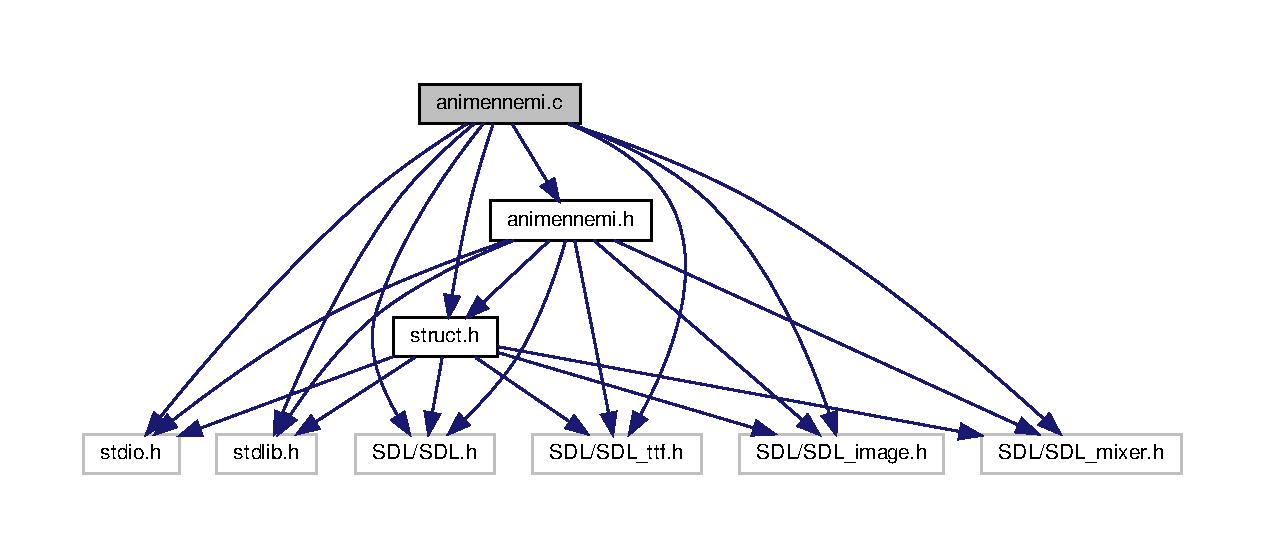
\includegraphics[width=350pt]{animennemi_8c__incl}
\end{center}
\end{figure}
\subsection*{Functions}
\begin{DoxyCompactItemize}
\item 
void \hyperlink{animennemi_8c_a449db8c266f1c795e8de1e9e9802f90b}{initialiserennemi} (\hyperlink{structennemi}{ennemi} $\ast$e)
\item 
void \hyperlink{animennemi_8c_ad429715f94be9c05e0f873efd01f62ff}{freesurfaceennemi} (\hyperlink{structennemi}{ennemi} $\ast$e)
\item 
void \hyperlink{animennemi_8c_aeaee7609b550df071dc748028caa3f97}{affichage\+\_\+ennemi} (\hyperlink{structennemi}{ennemi} e, S\+D\+L\+\_\+\+Surface $\ast$screen, \hyperlink{structbackground}{background} b)
\item 
void \hyperlink{animennemi_8c_a5b88fedc1de2481522fa32569e5b7393}{mvm\+\_\+alea\+\_\+enemi} (\hyperlink{structennemi}{ennemi} $\ast$e)
\end{DoxyCompactItemize}


\subsection{Function Documentation}
\mbox{\Hypertarget{animennemi_8c_aeaee7609b550df071dc748028caa3f97}\label{animennemi_8c_aeaee7609b550df071dc748028caa3f97}} 
\index{animennemi.\+c@{animennemi.\+c}!affichage\+\_\+ennemi@{affichage\+\_\+ennemi}}
\index{affichage\+\_\+ennemi@{affichage\+\_\+ennemi}!animennemi.\+c@{animennemi.\+c}}
\subsubsection{\texorpdfstring{affichage\+\_\+ennemi()}{affichage\_ennemi()}}
{\footnotesize\ttfamily void affichage\+\_\+ennemi (\begin{DoxyParamCaption}\item[{\hyperlink{structennemi}{ennemi}}]{e,  }\item[{S\+D\+L\+\_\+\+Surface $\ast$}]{screen,  }\item[{\hyperlink{structbackground}{background}}]{b }\end{DoxyParamCaption})}

Here is the call graph for this function\+:
\nopagebreak
\begin{figure}[H]
\begin{center}
\leavevmode
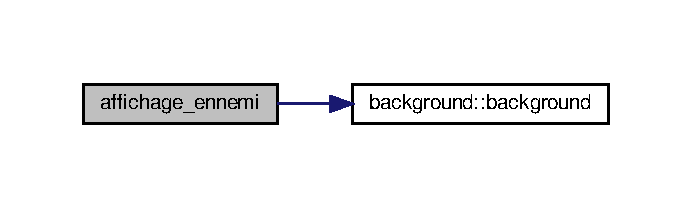
\includegraphics[width=332pt]{animennemi_8c_aeaee7609b550df071dc748028caa3f97_cgraph}
\end{center}
\end{figure}
Here is the caller graph for this function\+:
\nopagebreak
\begin{figure}[H]
\begin{center}
\leavevmode
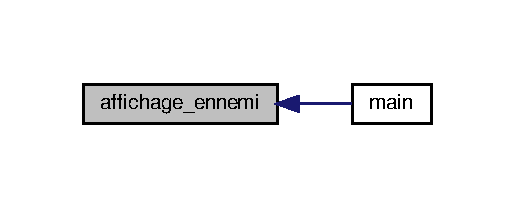
\includegraphics[width=247pt]{animennemi_8c_aeaee7609b550df071dc748028caa3f97_icgraph}
\end{center}
\end{figure}
\mbox{\Hypertarget{animennemi_8c_ad429715f94be9c05e0f873efd01f62ff}\label{animennemi_8c_ad429715f94be9c05e0f873efd01f62ff}} 
\index{animennemi.\+c@{animennemi.\+c}!freesurfaceennemi@{freesurfaceennemi}}
\index{freesurfaceennemi@{freesurfaceennemi}!animennemi.\+c@{animennemi.\+c}}
\subsubsection{\texorpdfstring{freesurfaceennemi()}{freesurfaceennemi()}}
{\footnotesize\ttfamily void freesurfaceennemi (\begin{DoxyParamCaption}\item[{\hyperlink{structennemi}{ennemi} $\ast$}]{e }\end{DoxyParamCaption})}

Here is the caller graph for this function\+:
\nopagebreak
\begin{figure}[H]
\begin{center}
\leavevmode
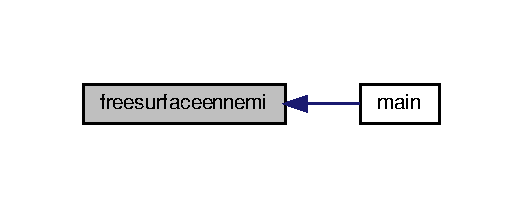
\includegraphics[width=251pt]{animennemi_8c_ad429715f94be9c05e0f873efd01f62ff_icgraph}
\end{center}
\end{figure}
\mbox{\Hypertarget{animennemi_8c_a449db8c266f1c795e8de1e9e9802f90b}\label{animennemi_8c_a449db8c266f1c795e8de1e9e9802f90b}} 
\index{animennemi.\+c@{animennemi.\+c}!initialiserennemi@{initialiserennemi}}
\index{initialiserennemi@{initialiserennemi}!animennemi.\+c@{animennemi.\+c}}
\subsubsection{\texorpdfstring{initialiserennemi()}{initialiserennemi()}}
{\footnotesize\ttfamily void initialiserennemi (\begin{DoxyParamCaption}\item[{\hyperlink{structennemi}{ennemi} $\ast$}]{e }\end{DoxyParamCaption})}

Here is the caller graph for this function\+:
\nopagebreak
\begin{figure}[H]
\begin{center}
\leavevmode
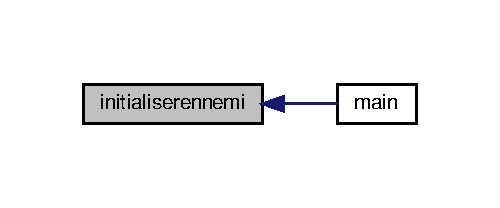
\includegraphics[width=240pt]{animennemi_8c_a449db8c266f1c795e8de1e9e9802f90b_icgraph}
\end{center}
\end{figure}
\mbox{\Hypertarget{animennemi_8c_a5b88fedc1de2481522fa32569e5b7393}\label{animennemi_8c_a5b88fedc1de2481522fa32569e5b7393}} 
\index{animennemi.\+c@{animennemi.\+c}!mvm\+\_\+alea\+\_\+enemi@{mvm\+\_\+alea\+\_\+enemi}}
\index{mvm\+\_\+alea\+\_\+enemi@{mvm\+\_\+alea\+\_\+enemi}!animennemi.\+c@{animennemi.\+c}}
\subsubsection{\texorpdfstring{mvm\+\_\+alea\+\_\+enemi()}{mvm\_alea\_enemi()}}
{\footnotesize\ttfamily void mvm\+\_\+alea\+\_\+enemi (\begin{DoxyParamCaption}\item[{\hyperlink{structennemi}{ennemi} $\ast$}]{e }\end{DoxyParamCaption})}

Here is the caller graph for this function\+:
\nopagebreak
\begin{figure}[H]
\begin{center}
\leavevmode
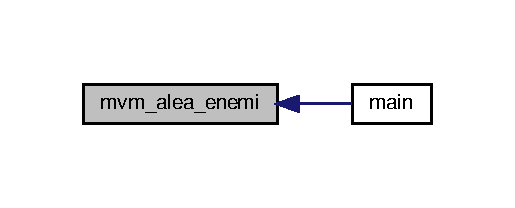
\includegraphics[width=247pt]{animennemi_8c_a5b88fedc1de2481522fa32569e5b7393_icgraph}
\end{center}
\end{figure}

\hypertarget{animennemi_8h}{}\section{animennemi.\+h File Reference}
\label{animennemi_8h}\index{animennemi.\+h@{animennemi.\+h}}
{\ttfamily \#include $<$stdio.\+h$>$}\newline
{\ttfamily \#include $<$stdlib.\+h$>$}\newline
{\ttfamily \#include \char`\"{}S\+D\+L/\+S\+D\+L.\+h\char`\"{}}\newline
{\ttfamily \#include \char`\"{}S\+D\+L/\+S\+D\+L\+\_\+image.\+h\char`\"{}}\newline
{\ttfamily \#include \char`\"{}S\+D\+L/\+S\+D\+L\+\_\+mixer.\+h\char`\"{}}\newline
{\ttfamily \#include \char`\"{}S\+D\+L/\+S\+D\+L\+\_\+ttf.\+h\char`\"{}}\newline
{\ttfamily \#include \char`\"{}struct.\+h\char`\"{}}\newline
Include dependency graph for animennemi.\+h\+:
\nopagebreak
\begin{figure}[H]
\begin{center}
\leavevmode
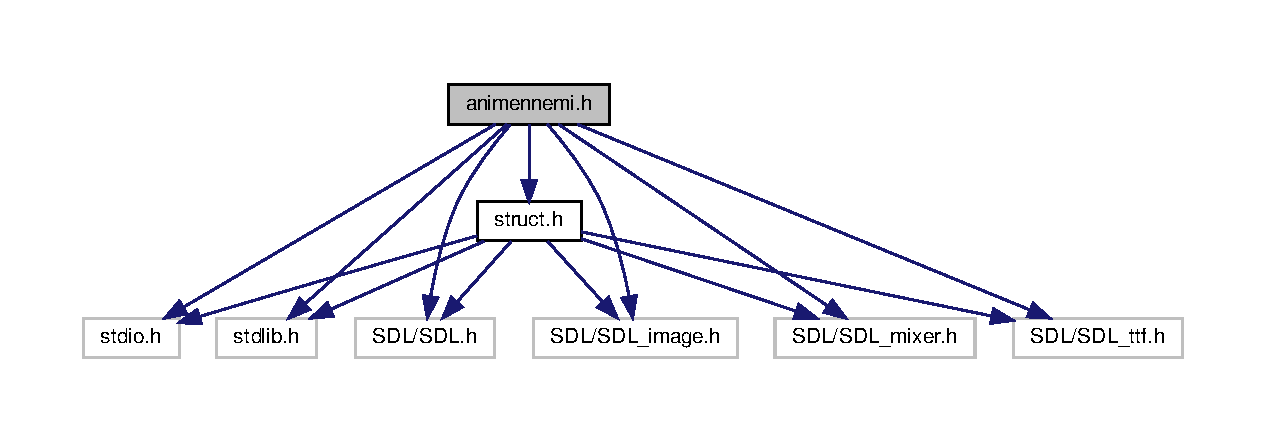
\includegraphics[width=350pt]{animennemi_8h__incl}
\end{center}
\end{figure}
This graph shows which files directly or indirectly include this file\+:
\nopagebreak
\begin{figure}[H]
\begin{center}
\leavevmode
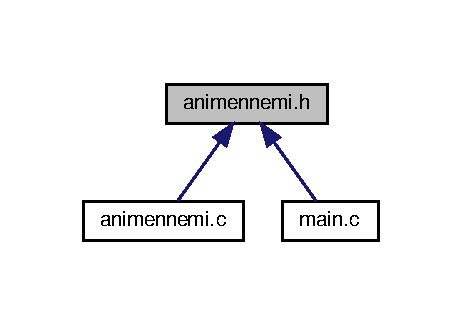
\includegraphics[width=222pt]{animennemi_8h__dep__incl}
\end{center}
\end{figure}
\subsection*{Data Structures}
\begin{DoxyCompactItemize}
\item 
struct \hyperlink{structbackground}{background}
\item 
struct \hyperlink{structennemi}{ennemi}
\end{DoxyCompactItemize}
\subsection*{Typedefs}
\begin{DoxyCompactItemize}
\item 
typedef struct \hyperlink{structbackground}{background} \hyperlink{animennemi_8h_ac7ec97684ccd0aaa88e134ebcc2478bb}{background}
\item 
typedef struct \hyperlink{structennemi}{ennemi} \hyperlink{animennemi_8h_ab7eb9415b369de28d9a91182c35b6fab}{ennemi}
\end{DoxyCompactItemize}
\subsection*{Functions}
\begin{DoxyCompactItemize}
\item 
void \hyperlink{animennemi_8h_a449db8c266f1c795e8de1e9e9802f90b}{initialiserennemi} (\hyperlink{structennemi}{ennemi} $\ast$e)
\item 
void \hyperlink{animennemi_8h_ad429715f94be9c05e0f873efd01f62ff}{freesurfaceennemi} (\hyperlink{structennemi}{ennemi} $\ast$e)
\item 
void \hyperlink{animennemi_8h_aeaee7609b550df071dc748028caa3f97}{affichage\+\_\+ennemi} (\hyperlink{structennemi}{ennemi} e, S\+D\+L\+\_\+\+Surface $\ast$screen, \hyperlink{structbackground}{background} b)
\item 
void \hyperlink{animennemi_8h_a5b88fedc1de2481522fa32569e5b7393}{mvm\+\_\+alea\+\_\+enemi} (\hyperlink{structennemi}{ennemi} $\ast$e)
\end{DoxyCompactItemize}


\subsection{Typedef Documentation}
\mbox{\Hypertarget{animennemi_8h_ac7ec97684ccd0aaa88e134ebcc2478bb}\label{animennemi_8h_ac7ec97684ccd0aaa88e134ebcc2478bb}} 
\index{animennemi.\+h@{animennemi.\+h}!background@{background}}
\index{background@{background}!animennemi.\+h@{animennemi.\+h}}
\subsubsection{\texorpdfstring{background}{background}}
{\footnotesize\ttfamily typedef struct \hyperlink{structbackground}{background} \hyperlink{structbackground}{background}}

\mbox{\Hypertarget{animennemi_8h_ab7eb9415b369de28d9a91182c35b6fab}\label{animennemi_8h_ab7eb9415b369de28d9a91182c35b6fab}} 
\index{animennemi.\+h@{animennemi.\+h}!ennemi@{ennemi}}
\index{ennemi@{ennemi}!animennemi.\+h@{animennemi.\+h}}
\subsubsection{\texorpdfstring{ennemi}{ennemi}}
{\footnotesize\ttfamily typedef struct \hyperlink{structennemi}{ennemi} \hyperlink{structennemi}{ennemi}}



\subsection{Function Documentation}
\mbox{\Hypertarget{animennemi_8h_aeaee7609b550df071dc748028caa3f97}\label{animennemi_8h_aeaee7609b550df071dc748028caa3f97}} 
\index{animennemi.\+h@{animennemi.\+h}!affichage\+\_\+ennemi@{affichage\+\_\+ennemi}}
\index{affichage\+\_\+ennemi@{affichage\+\_\+ennemi}!animennemi.\+h@{animennemi.\+h}}
\subsubsection{\texorpdfstring{affichage\+\_\+ennemi()}{affichage\_ennemi()}}
{\footnotesize\ttfamily void affichage\+\_\+ennemi (\begin{DoxyParamCaption}\item[{\hyperlink{structennemi}{ennemi}}]{e,  }\item[{S\+D\+L\+\_\+\+Surface $\ast$}]{screen,  }\item[{\hyperlink{structbackground}{background}}]{b }\end{DoxyParamCaption})}

Here is the call graph for this function\+:
\nopagebreak
\begin{figure}[H]
\begin{center}
\leavevmode
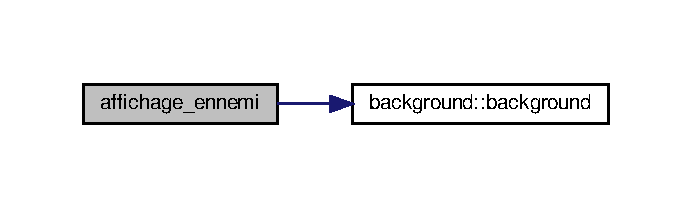
\includegraphics[width=332pt]{animennemi_8h_aeaee7609b550df071dc748028caa3f97_cgraph}
\end{center}
\end{figure}
Here is the caller graph for this function\+:
\nopagebreak
\begin{figure}[H]
\begin{center}
\leavevmode
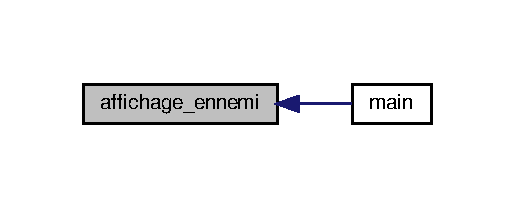
\includegraphics[width=247pt]{animennemi_8h_aeaee7609b550df071dc748028caa3f97_icgraph}
\end{center}
\end{figure}
\mbox{\Hypertarget{animennemi_8h_ad429715f94be9c05e0f873efd01f62ff}\label{animennemi_8h_ad429715f94be9c05e0f873efd01f62ff}} 
\index{animennemi.\+h@{animennemi.\+h}!freesurfaceennemi@{freesurfaceennemi}}
\index{freesurfaceennemi@{freesurfaceennemi}!animennemi.\+h@{animennemi.\+h}}
\subsubsection{\texorpdfstring{freesurfaceennemi()}{freesurfaceennemi()}}
{\footnotesize\ttfamily void freesurfaceennemi (\begin{DoxyParamCaption}\item[{\hyperlink{structennemi}{ennemi} $\ast$}]{e }\end{DoxyParamCaption})}

Here is the caller graph for this function\+:
\nopagebreak
\begin{figure}[H]
\begin{center}
\leavevmode
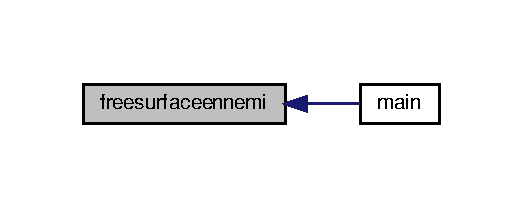
\includegraphics[width=251pt]{animennemi_8h_ad429715f94be9c05e0f873efd01f62ff_icgraph}
\end{center}
\end{figure}
\mbox{\Hypertarget{animennemi_8h_a449db8c266f1c795e8de1e9e9802f90b}\label{animennemi_8h_a449db8c266f1c795e8de1e9e9802f90b}} 
\index{animennemi.\+h@{animennemi.\+h}!initialiserennemi@{initialiserennemi}}
\index{initialiserennemi@{initialiserennemi}!animennemi.\+h@{animennemi.\+h}}
\subsubsection{\texorpdfstring{initialiserennemi()}{initialiserennemi()}}
{\footnotesize\ttfamily void initialiserennemi (\begin{DoxyParamCaption}\item[{\hyperlink{structennemi}{ennemi} $\ast$}]{e }\end{DoxyParamCaption})}

Here is the caller graph for this function\+:
\nopagebreak
\begin{figure}[H]
\begin{center}
\leavevmode
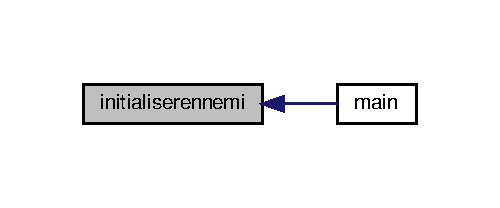
\includegraphics[width=240pt]{animennemi_8h_a449db8c266f1c795e8de1e9e9802f90b_icgraph}
\end{center}
\end{figure}
\mbox{\Hypertarget{animennemi_8h_a5b88fedc1de2481522fa32569e5b7393}\label{animennemi_8h_a5b88fedc1de2481522fa32569e5b7393}} 
\index{animennemi.\+h@{animennemi.\+h}!mvm\+\_\+alea\+\_\+enemi@{mvm\+\_\+alea\+\_\+enemi}}
\index{mvm\+\_\+alea\+\_\+enemi@{mvm\+\_\+alea\+\_\+enemi}!animennemi.\+h@{animennemi.\+h}}
\subsubsection{\texorpdfstring{mvm\+\_\+alea\+\_\+enemi()}{mvm\_alea\_enemi()}}
{\footnotesize\ttfamily void mvm\+\_\+alea\+\_\+enemi (\begin{DoxyParamCaption}\item[{\hyperlink{structennemi}{ennemi} $\ast$}]{e }\end{DoxyParamCaption})}

Here is the caller graph for this function\+:
\nopagebreak
\begin{figure}[H]
\begin{center}
\leavevmode
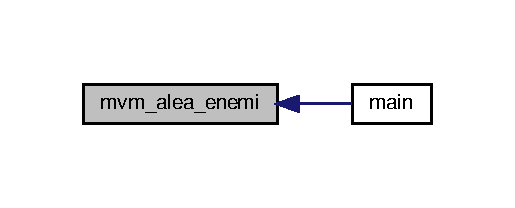
\includegraphics[width=247pt]{animennemi_8h_a5b88fedc1de2481522fa32569e5b7393_icgraph}
\end{center}
\end{figure}

\hypertarget{horloge_8c}{}\section{horloge.\+c File Reference}
\label{horloge_8c}\index{horloge.\+c@{horloge.\+c}}
{\ttfamily \#include \char`\"{}ennemi.\+h\char`\"{}}\newline
{\ttfamily \#include $<$stdio.\+h$>$}\newline
{\ttfamily \#include $<$stdlib.\+h$>$}\newline
{\ttfamily \#include \char`\"{}S\+D\+L/\+S\+D\+L.\+h\char`\"{}}\newline
{\ttfamily \#include \char`\"{}S\+D\+L/\+S\+D\+L\+\_\+image.\+h\char`\"{}}\newline
{\ttfamily \#include \char`\"{}S\+D\+L/\+S\+D\+L\+\_\+mixer.\+h\char`\"{}}\newline
{\ttfamily \#include \char`\"{}S\+D\+L/\+S\+D\+L\+\_\+ttf.\+h\char`\"{}}\newline
{\ttfamily \#include $<$time.\+h$>$}\newline
Include dependency graph for horloge.\+c\+:
\nopagebreak
\begin{figure}[H]
\begin{center}
\leavevmode
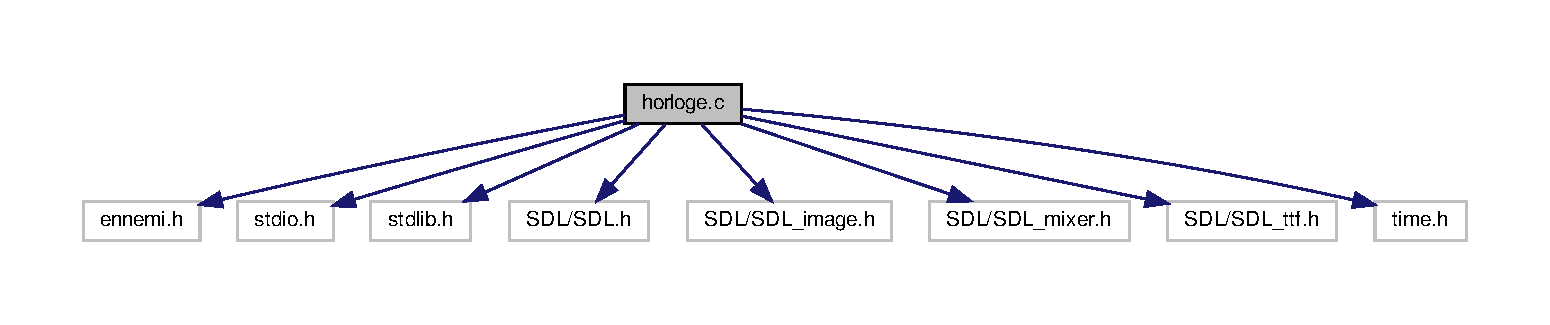
\includegraphics[width=350pt]{horloge_8c__incl}
\end{center}
\end{figure}
\subsection*{Functions}
\begin{DoxyCompactItemize}
\item 
S\+D\+L\+\_\+\+Surface $\ast$ \hyperlink{horloge_8c_ad044c3f22540eeec6d9f3e57ada0a7c4}{game\+Time} (\hyperlink{structtimer}{timer} $\ast$t)
\end{DoxyCompactItemize}


\subsection{Function Documentation}
\mbox{\Hypertarget{horloge_8c_ad044c3f22540eeec6d9f3e57ada0a7c4}\label{horloge_8c_ad044c3f22540eeec6d9f3e57ada0a7c4}} 
\index{horloge.\+c@{horloge.\+c}!game\+Time@{game\+Time}}
\index{game\+Time@{game\+Time}!horloge.\+c@{horloge.\+c}}
\subsubsection{\texorpdfstring{game\+Time()}{gameTime()}}
{\footnotesize\ttfamily S\+D\+L\+\_\+\+Surface$\ast$ game\+Time (\begin{DoxyParamCaption}\item[{\hyperlink{structtimer}{timer} $\ast$}]{t }\end{DoxyParamCaption})}


\hypertarget{horloge_8h}{}\section{horloge.\+h File Reference}
\label{horloge_8h}\index{horloge.\+h@{horloge.\+h}}
{\ttfamily \#include $<$stdio.\+h$>$}\newline
{\ttfamily \#include $<$stdlib.\+h$>$}\newline
{\ttfamily \#include \char`\"{}S\+D\+L/\+S\+D\+L.\+h\char`\"{}}\newline
{\ttfamily \#include \char`\"{}S\+D\+L/\+S\+D\+L\+\_\+image.\+h\char`\"{}}\newline
{\ttfamily \#include \char`\"{}S\+D\+L/\+S\+D\+L\+\_\+mixer.\+h\char`\"{}}\newline
{\ttfamily \#include \char`\"{}S\+D\+L/\+S\+D\+L\+\_\+ttf.\+h\char`\"{}}\newline
{\ttfamily \#include $<$time.\+h$>$}\newline
Include dependency graph for horloge.\+h\+:
\nopagebreak
\begin{figure}[H]
\begin{center}
\leavevmode
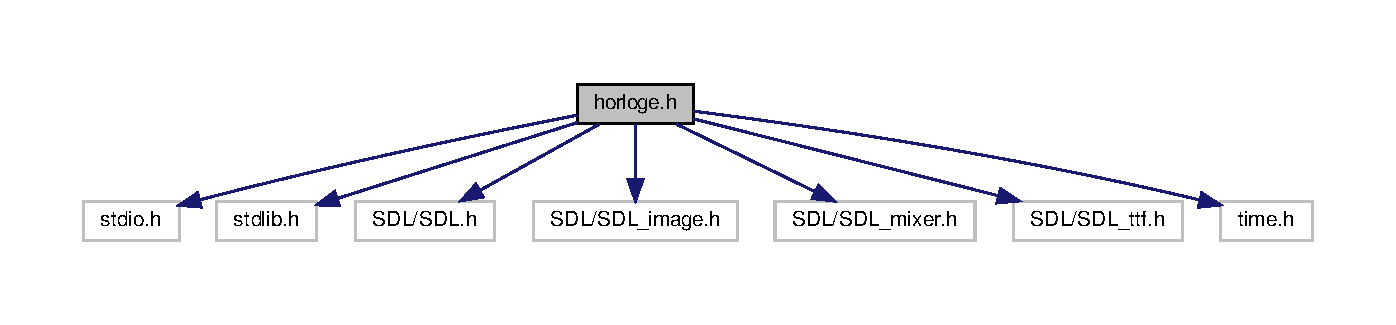
\includegraphics[width=350pt]{horloge_8h__incl}
\end{center}
\end{figure}
\subsection*{Data Structures}
\begin{DoxyCompactItemize}
\item 
struct \hyperlink{structtimer}{timer}
\end{DoxyCompactItemize}
\subsection*{Typedefs}
\begin{DoxyCompactItemize}
\item 
typedef struct \hyperlink{structtimer}{timer} \hyperlink{horloge_8h_a1ee61f616609d1fee9359d9f9c3a97ec}{timer}
\end{DoxyCompactItemize}
\subsection*{Functions}
\begin{DoxyCompactItemize}
\item 
S\+D\+L\+\_\+\+Surface $\ast$ \hyperlink{horloge_8h_ad044c3f22540eeec6d9f3e57ada0a7c4}{game\+Time} (\hyperlink{structtimer}{timer} $\ast$t)
\end{DoxyCompactItemize}


\subsection{Typedef Documentation}
\mbox{\Hypertarget{horloge_8h_a1ee61f616609d1fee9359d9f9c3a97ec}\label{horloge_8h_a1ee61f616609d1fee9359d9f9c3a97ec}} 
\index{horloge.\+h@{horloge.\+h}!timer@{timer}}
\index{timer@{timer}!horloge.\+h@{horloge.\+h}}
\subsubsection{\texorpdfstring{timer}{timer}}
{\footnotesize\ttfamily typedef struct \hyperlink{structtimer}{timer} \hyperlink{structtimer}{timer}}



\subsection{Function Documentation}
\mbox{\Hypertarget{horloge_8h_ad044c3f22540eeec6d9f3e57ada0a7c4}\label{horloge_8h_ad044c3f22540eeec6d9f3e57ada0a7c4}} 
\index{horloge.\+h@{horloge.\+h}!game\+Time@{game\+Time}}
\index{game\+Time@{game\+Time}!horloge.\+h@{horloge.\+h}}
\subsubsection{\texorpdfstring{game\+Time()}{gameTime()}}
{\footnotesize\ttfamily S\+D\+L\+\_\+\+Surface$\ast$ game\+Time (\begin{DoxyParamCaption}\item[{\hyperlink{structtimer}{timer} $\ast$}]{t }\end{DoxyParamCaption})}


\hypertarget{main_8c}{}\section{main.\+c File Reference}
\label{main_8c}\index{main.\+c@{main.\+c}}
{\ttfamily \#include $<$stdio.\+h$>$}\newline
{\ttfamily \#include $<$stdlib.\+h$>$}\newline
{\ttfamily \#include $<$S\+D\+L/\+S\+D\+L.\+h$>$}\newline
{\ttfamily \#include $<$S\+D\+L/\+S\+D\+L\+\_\+image.\+h$>$}\newline
{\ttfamily \#include $<$S\+D\+L/\+S\+D\+L\+\_\+ttf.\+h$>$}\newline
{\ttfamily \#include \char`\"{}S\+D\+L/\+S\+D\+L\+\_\+mixer.\+h\char`\"{}}\newline
{\ttfamily \#include \char`\"{}menu.\+h\char`\"{}}\newline
Include dependency graph for main.\+c\+:
\nopagebreak
\begin{figure}[H]
\begin{center}
\leavevmode
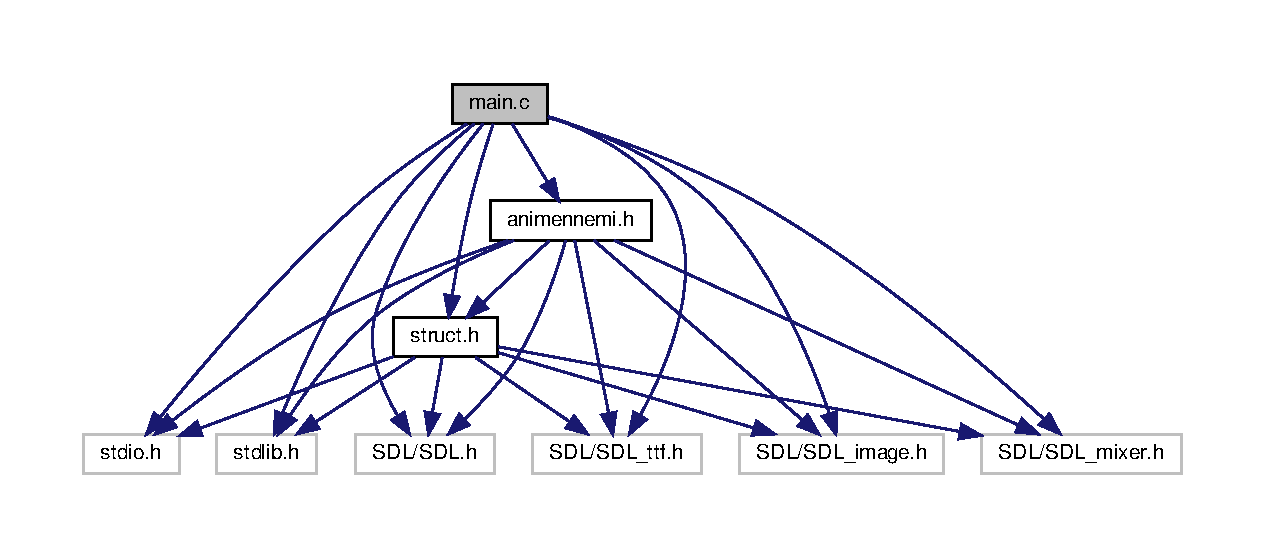
\includegraphics[width=350pt]{main_8c__incl}
\end{center}
\end{figure}
\subsection*{Functions}
\begin{DoxyCompactItemize}
\item 
int \hyperlink{main_8c_ae66f6b31b5ad750f1fe042a706a4e3d4}{main} ()
\end{DoxyCompactItemize}


\subsection{Function Documentation}
\mbox{\Hypertarget{main_8c_ae66f6b31b5ad750f1fe042a706a4e3d4}\label{main_8c_ae66f6b31b5ad750f1fe042a706a4e3d4}} 
\index{main.\+c@{main.\+c}!main@{main}}
\index{main@{main}!main.\+c@{main.\+c}}
\subsubsection{\texorpdfstring{main()}{main()}}
{\footnotesize\ttfamily int main (\begin{DoxyParamCaption}{ }\end{DoxyParamCaption})}

Here is the call graph for this function\+:
\nopagebreak
\begin{figure}[H]
\begin{center}
\leavevmode
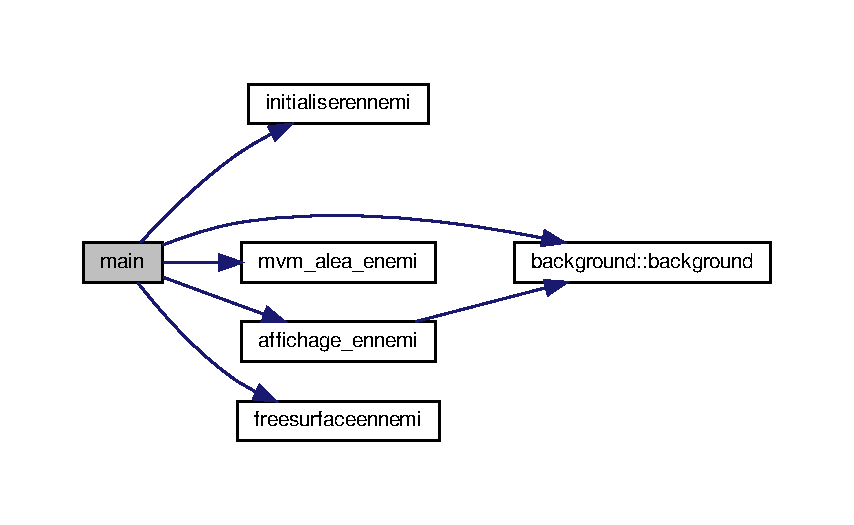
\includegraphics[width=350pt]{main_8c_ae66f6b31b5ad750f1fe042a706a4e3d4_cgraph}
\end{center}
\end{figure}

\hypertarget{struct_8h}{}\section{struct.\+h File Reference}
\label{struct_8h}\index{struct.\+h@{struct.\+h}}
{\ttfamily \#include $<$stdio.\+h$>$}\newline
{\ttfamily \#include $<$stdlib.\+h$>$}\newline
{\ttfamily \#include \char`\"{}S\+D\+L/\+S\+D\+L.\+h\char`\"{}}\newline
{\ttfamily \#include \char`\"{}S\+D\+L/\+S\+D\+L\+\_\+image.\+h\char`\"{}}\newline
{\ttfamily \#include \char`\"{}S\+D\+L/\+S\+D\+L\+\_\+mixer.\+h\char`\"{}}\newline
{\ttfamily \#include \char`\"{}S\+D\+L/\+S\+D\+L\+\_\+ttf.\+h\char`\"{}}\newline
Include dependency graph for struct.\+h\+:
\nopagebreak
\begin{figure}[H]
\begin{center}
\leavevmode
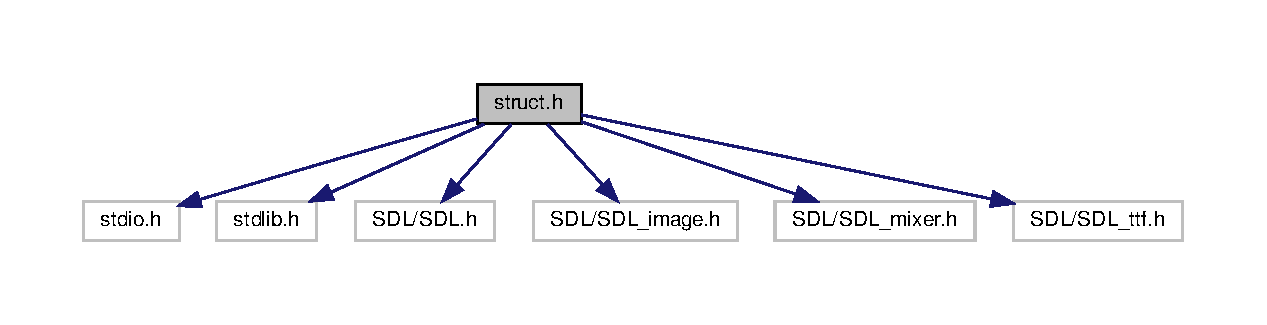
\includegraphics[width=350pt]{struct_8h__incl}
\end{center}
\end{figure}
This graph shows which files directly or indirectly include this file\+:
\nopagebreak
\begin{figure}[H]
\begin{center}
\leavevmode
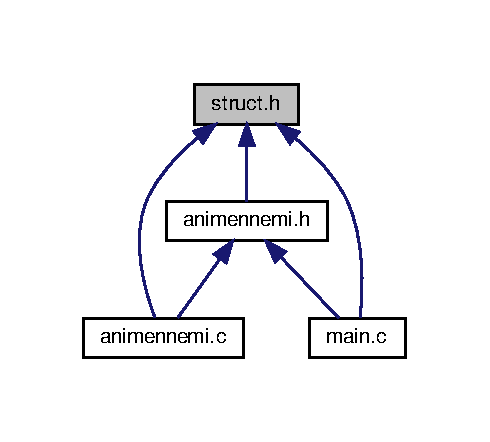
\includegraphics[width=235pt]{struct_8h__dep__incl}
\end{center}
\end{figure}
\subsection*{Data Structures}
\begin{DoxyCompactItemize}
\item 
struct \hyperlink{structbackground}{background}
\item 
struct \hyperlink{structvie}{vie}
\item 
struct \hyperlink{structscore}{score}
\item 
struct \hyperlink{structpersonnage}{personnage}
\item 
struct \hyperlink{structennemi}{ennemi}
\end{DoxyCompactItemize}
\subsection*{Typedefs}
\begin{DoxyCompactItemize}
\item 
typedef struct \hyperlink{structbackground}{background} \hyperlink{struct_8h_ac7ec97684ccd0aaa88e134ebcc2478bb}{background}
\item 
typedef struct \hyperlink{structvie}{vie} \hyperlink{struct_8h_a5a50eadb578d4b4b9db54fdffc9b3c48}{vie}
\item 
typedef struct \hyperlink{structscore}{score} \hyperlink{struct_8h_a1240ca29fa6f99334b17271ea026bc91}{score}
\item 
typedef struct \hyperlink{structpersonnage}{personnage} \hyperlink{struct_8h_a22ea6c21be7b6540d95f47b6ad40ffa6}{personnage}
\item 
typedef struct \hyperlink{structennemi}{ennemi} \hyperlink{struct_8h_ab7eb9415b369de28d9a91182c35b6fab}{ennemi}
\end{DoxyCompactItemize}


\subsection{Typedef Documentation}
\mbox{\Hypertarget{struct_8h_ac7ec97684ccd0aaa88e134ebcc2478bb}\label{struct_8h_ac7ec97684ccd0aaa88e134ebcc2478bb}} 
\index{struct.\+h@{struct.\+h}!background@{background}}
\index{background@{background}!struct.\+h@{struct.\+h}}
\subsubsection{\texorpdfstring{background}{background}}
{\footnotesize\ttfamily typedef struct \hyperlink{structbackground}{background} \hyperlink{structbackground}{background}}

\mbox{\Hypertarget{struct_8h_ab7eb9415b369de28d9a91182c35b6fab}\label{struct_8h_ab7eb9415b369de28d9a91182c35b6fab}} 
\index{struct.\+h@{struct.\+h}!ennemi@{ennemi}}
\index{ennemi@{ennemi}!struct.\+h@{struct.\+h}}
\subsubsection{\texorpdfstring{ennemi}{ennemi}}
{\footnotesize\ttfamily typedef struct \hyperlink{structennemi}{ennemi} \hyperlink{structennemi}{ennemi}}

\mbox{\Hypertarget{struct_8h_a22ea6c21be7b6540d95f47b6ad40ffa6}\label{struct_8h_a22ea6c21be7b6540d95f47b6ad40ffa6}} 
\index{struct.\+h@{struct.\+h}!personnage@{personnage}}
\index{personnage@{personnage}!struct.\+h@{struct.\+h}}
\subsubsection{\texorpdfstring{personnage}{personnage}}
{\footnotesize\ttfamily typedef struct \hyperlink{structpersonnage}{personnage}  \hyperlink{structpersonnage}{personnage}}

\mbox{\Hypertarget{struct_8h_a1240ca29fa6f99334b17271ea026bc91}\label{struct_8h_a1240ca29fa6f99334b17271ea026bc91}} 
\index{struct.\+h@{struct.\+h}!score@{score}}
\index{score@{score}!struct.\+h@{struct.\+h}}
\subsubsection{\texorpdfstring{score}{score}}
{\footnotesize\ttfamily typedef struct \hyperlink{structscore}{score} \hyperlink{structscore}{score}}

\mbox{\Hypertarget{struct_8h_a5a50eadb578d4b4b9db54fdffc9b3c48}\label{struct_8h_a5a50eadb578d4b4b9db54fdffc9b3c48}} 
\index{struct.\+h@{struct.\+h}!vie@{vie}}
\index{vie@{vie}!struct.\+h@{struct.\+h}}
\subsubsection{\texorpdfstring{vie}{vie}}
{\footnotesize\ttfamily typedef struct \hyperlink{structvie}{vie} \hyperlink{structvie}{vie}}


%--- End generated contents ---

% Index
\backmatter
\newpage
\phantomsection
\clearemptydoublepage
\addcontentsline{toc}{chapter}{Index}
\printindex

\end{document}
